%\chapter{Differential branching fraction of the rare \Lb\to\Lz\mumu decay}
\chapter{Differential branching fraction of $\protect\Lb\to\Lz\mumu$}
\label{sec:Lmumu_intro}

The rare $\Lb\to\Lz\mumu$ decay is a FCNC process governed by the $\bquark \to \squark\mumu$ quark
level transition. In the SM this decay proceeds only through loop diagrams (electroweak penguin and \W box)
as discussed in Sec.~\ref{sec:RD_theory}, and therefore it is highly sensitive to new particles entering the loops. 
%Moreover, as the final state contains only a single long-lived hadron,
%the hadronic physics is easier to handle than in fully hadronic decays.
%\begin{figure}[hbt]
%\centering
%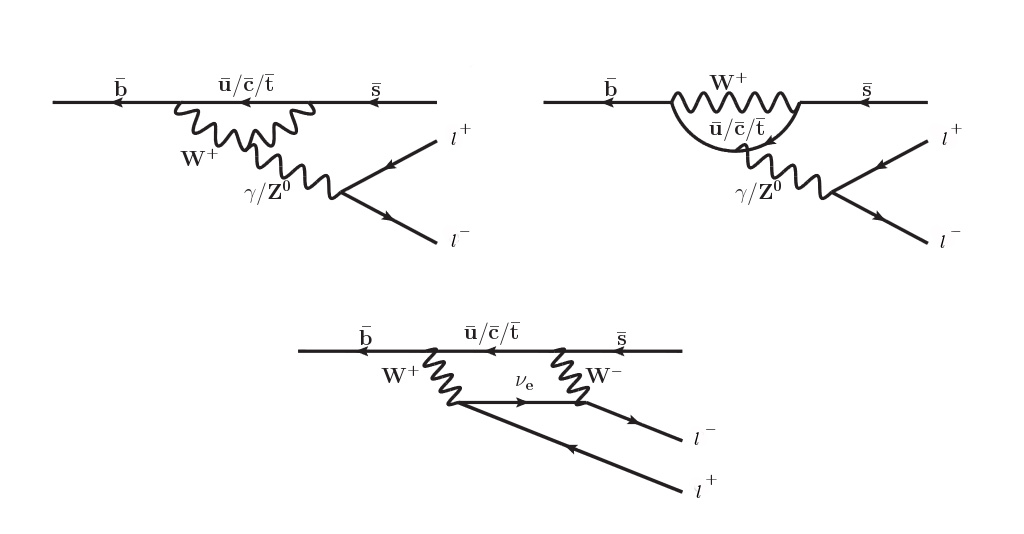
\includegraphics[width=0.8\textwidth]{Lmumu/figs/penguins3.png}
%\caption{Loop Feynmann diagrams for the rare $b \rightarrow s $ decay.}
%\label{fig:penguins}
%\end{figure}
%
Interest in \Lb baryon decays arises from two important facts.
First of all, the \Lb has non-zero initial spin, which allows us to extract information about the helicity structure
of the underlying Hamiltonian that cannot be obtained from the meson decays~\cite{Hiller:2007ur,Mannel:1997xy}.
Secondly, the \Lb baryon can be considered to a first approximation as being composed of a heavy 
quark and a light di-quark, therefore the hadronic physics differs significantly from similar meson decays.
This provides the possibility to better understand and test the hadronic physics in the theory,
which could yield improved understanding that would also be relevant for the meson case.

With respect to \Bz decays going though the same transitions, such as \BdToKstmm, \Lb decays can provide independent
confirmations of the results as they involve the same operators but different hadronic matrix elements.
Furthermore, \Lz baryons decays weakly, which results in complementary constraints with respect to \Bz decays.
Finally, the narrow width approximation, used in theoretical calculations, is fully applicable in the \Lb case,
which has $\Gamma_{\Lb} \sim 2.5 \cdot 10^{-6}$ \ev. This is not the case for \BdToKstmm decays because
the contribution from the non-resonant channel $\decay{\Bz}{K\pi\mumu}$ is unconstrained.

The theory of the $\Lb\to\Lz\mumu$ decays was widely considered both in the context of the SM and in different
new physics scenarios~\cite{Aslam:2008hp,Wang:2008sm,Huang:1998ek,Chen:2001ki,Chen:2001zc,Chen:2001sj,
Zolfagharpour:2007eh,Mott:2011cx,Aliev:2010uy,Mohanta:2010eb,Sahoo:2011yb}.
All authors start from the same effective Hamiltonian outlined in Sec.~\ref{sec:Effective_Hamiltonian}. 
However, form factors, describing hadronic physics are not as well-developed as for the meson case 
because there are fewer experimental constraints. This leads to a relatively
large spread in predicted branching fractions. For these reasons an interesting quantity to study is the differential 
branching fraction as a function of \qsq. This still suffers from the limited knowledge of form factors but, as different 
approaches to form factors calculations are applicable in different \qsq regions, it allows a more meaningful comparison with theory.

Experimentally, the $\Lb\to\Lz\mumu$ decay was observed for the first time in 2011 by the CDF 
collaboration~\cite{Aaltonen:2011qs}, with a signal yield of $24\pm5$ events, and later updated in preliminary form using
their full statistics~\cite{Behari:2013xc}. CDF observed the signal only in the \qsq region above the square of the \psitwos mass.
The latter measurement using their full statistics yields $\mathcal{B}($\Lb\to\Lz\mumu$) =[1.95\pm0.34(\mathrm{stat})\pm0.61(\mathrm{syst})]\times 10^{-6}$.
Recently, the decay was also observed at LHCb~\cite{LHCb-PAPER-2013-025} with a yield of $78\pm12$ signal events
using 1~\invfb of integrated luminosity collected in 2011. The signal was also found only in the high \qsq region, above $m^2_{\psitwos}$.
The LHCb result for the branching fraction relative to the $J/\psi\Lambda$ decay, which is used as a normalisation channel, is 
%
\begin{equation*}
\frac{\mathcal{B}(\Lb\to\Lz\mumu)}{\mathcal{B}(\Lb\to\jpsi\Lz)}=[1.54 \pm 0.30 ~(\mathrm{stat})~ \pm 0.20 ~(\mathrm{syst})~ \pm 0.02 ~(\mathrm{norm})]\times 10^{-3} 
\end{equation*}
and for absolute branching fraction,
\begin{equation*}
\mathcal{B}(\Lb\to\Lz\mumu) =[0.96 \pm 0.16 ~(\mathrm{stat})~ \pm 0.13 ~(\mathrm{syst})~ \pm 0.21 ~(\mathrm{norm})]\times 10^{-6}.
\end{equation*}

This chapter describes the measurement of the differential branching fraction
of the $\Lb\to\Lz\mumu$ decay using 3~\invfb of $pp$ collisions collected by the LHCb experiment in 2011 and 2012.
%Furthermore, in the next chapter an angular analysis of these decays is performed for the first time, measuring observables
%including the forward-backward asymmetries in the leptonic and hadronic systems.

\section{Analysis strategy and \qsq regions}
\label{sec:Lb_q2choice}

A typical \qsq spectrum of $\bquark\to\squark\ll$ decays was shown in Fig.~\ref{fig:q2spectrum}.
This is characterised by the presence of the photon pole at low \qsq and the narrow peaks of the \jpsi and \psitwos 
resonances at intermediate values of \qsq. In the analysis, $\Lb\to\jpsi\Lz$ decays, in which the \jpsi decays into two muons
 and therefore has the same final state as the signal, are used as the normalisation channel. The rare and normalisation 
 channels are naturally distinguished by the \qsq intervals in which they are reconstructed. 
The \Lz decay mode into a pion and a proton, $\Lz\to p\pi$, is always used to reconstruct the decays. 
% and the branching fraction measurement is given in relative form to limit systematic uncertainties. 
The intervals in which the rare channel is studied are:
\begin{itemize}
\item $0.1 < \qsq < 8$ \gevgevcccc, where the signal is unobserved and the selection 
is optimised to observe the signal. The upper bound of this interval is chosen to be sufficiently 
far from the \jpsi radiative tail at low masses and reduce its contamination into the rare sample;
\item $11 < \qsq < 12.5$ \gevgevcccc, between two charmonium resonances, and 
\item $\qsq>15$ \gevgevcccc, above \psitwos.
\end{itemize}
The first interval is referred to as ``low \qsq" region, below the \jpsi resonance ($\qsq < 8$ \gevgevcccc),
and the other two as ``high \qsq" regions, above the \jpsi resonance ($\qsq > 11$ \gevgevcccc).
%In the latter two intervals the selection is optimised to maximise the yield which is particularly important
%for a stable angular analysis. 
The above regions are then sub-divided into smaller intervals, as the available 
statistics allows, which results in $\sim 2$ \gevgevcccc wide bins. The binning used is the following:
\begin{equation}
[0.1, 2.0, 4.0, 6.0, 8.0], \jpsi, [11.0, 12.5], \psitwos, [15.0, 16.0, 18.0, 20.0].
\end{equation}

In addition the result is also provided in two integrated regions:
\begin{itemize}
\item 1.1-6.0 \gevgevcccc: this interval is theoretically clean since it is far from the
photon pole, which dominates at low \qsq values, reducing the sensitivity to new physics contributions.
The lower bound of this interval it chosen to exclude the possible contribution from
from the $\phi$ resonance, which appears at $\sim1$~\gevgevcccc. The upper bound of the interval
is chosen to exclude completely a small contribution from the \jpsi resonance that leaks
below 8~\gevgevcccc.
\item 15.0-20.0 \gevgevcccc: this interval is the one that is expected to contain most of the
rare decays and it is used as a natural cross check that the analysis is stable when performed in smaller bins.
\end{itemize}

\section{Candidate types}

This analysis deals with \Lz baryons, which have a lifetime of \mbox{$(2.632 \pm 0.020 ) \times 10^{-10}$ s~\cite{PDG2014}}.
These are considered long-lived particles in particle physics terms and can travel several metres into the
detector generating well distinguished secondary vertices.
In LHCb, \Lz baryons can be reconstructed from tracks either with or without hits in the VeLo (see Sec.~\ref{sec:tracking}) and
therefore two candidates types are defined as follows:

\begin{itemize}
\item {\bf Downstream candidates}: built from tracks without hits in the VeLo, 
``downstream tracks", also denoted as ``DD".
\item {\bf Long candidates}: built from tracks which have hits in the VeLo, ``long tracks".
These candidates, also denoted as ``LL", are characterised by a better momentum resolution
than downstream tracks thanks to the longer lever arm available to their tracks.
\end{itemize}

Figure~\ref{fig:track_types} shows the two types of candidates used in the analysis,
together with other possible track types in LHCb, which are not used in this analysis.
As the long and downstream candidate categories are characterised by different resolutions and 
kinematic properties, the analysis is performed separately on the two samples and the results are then combined.

\begin{figure}[hbt]
\centering
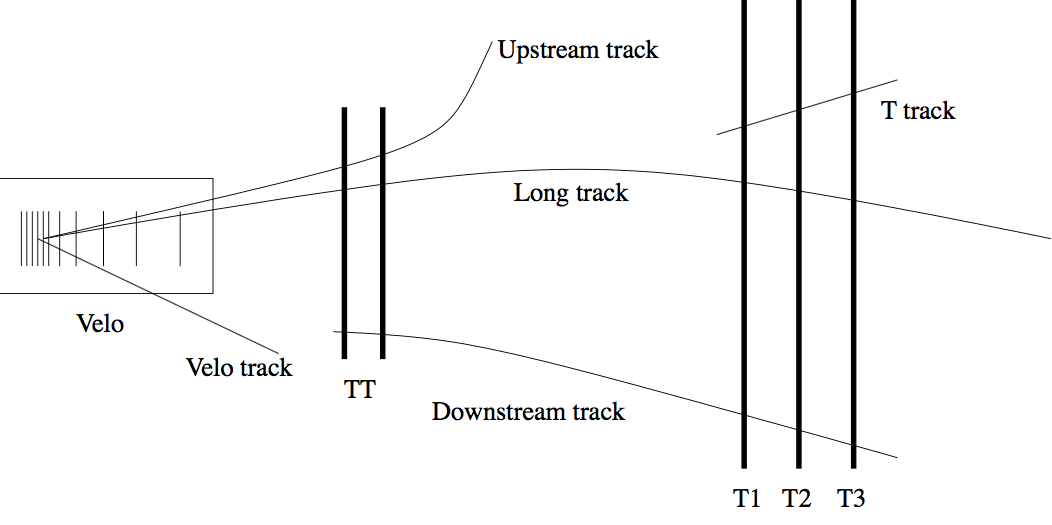
\includegraphics[width=0.8\textwidth,trim=0cm 0cm 0cm 5mm,]{Lmumu/figs/track_types.png}
\caption{Representation of possible track types in LHCb. Candidates built from ``long" and 
``downstream" tracks are used in this analysis~\cite{Alves:2008zz}.}
\label{fig:track_types}
\end{figure}
 
\section{Simulation}
\label{sec:Lb_simulation}

Samples of simulated events are needed in order to train the multivariate classifier
(see Sec.~\ref{sec:Lb_mva}), calculate the selection efficiency and study possible backgrounds;
in particular for this analysis samples of $\sim 2$ millions $\Lb\to\jpsi\Lz$ and 
$\sim 5$ millions $\Lb\to\Lz\mumu$ simulated events are used.
Samples of simulated $\Bz\ra\jpsi\KS$, $\Bz\ra\KS\mumu$ and $B^{+} \ra\mumu K^{*+}$
events are also used to study backgrounds from these decays. The events are generated using
$\textsc{Pythia}8$; hadronic particles are decayed using $\textsc{EvtGen}$ and $\textsc{Geant4}$ is used to simulate
the interaction of final state particles with the detector. Simulated events are then
reconstructed by the same reconstruction software that is used for real data. The L0 hardware
trigger is emulated in the simulation, while for the software stage, HLT
(see Sec.~\ref{sec:det_trigger}), the same code can be used as for data.
Events are simulated using both 2011 and 2012 beam and detector conditions, in the same proportion as
recorded data. While the simulation gives a generally good description of data, some discrepancies remain.
It is important that the simulation gives an accurate description of the data, 
in particular for the extraction of efficiencies. The next sections therefore 
describe corrections applied to the simulation in order to provide a better description of data.
In Appendix~\ref{app:MC_data_comp} data distributions are compared with simulated ones for
variables relevant to this analysis.

\subsection{Decay Model}
\label{decaymodel}

Little is known about the decay structure of \Lb decays and therefore the simulation software generates events
according to the phase space given by the available kinematics. To include a reasonably realistic \qsq dependence,
the simulation is weighted using decay amplitudes based on the predictions in Ref.~\cite{Gutsche:2013pp}.
Equations in this paper are for the case of unpolarised \Lb production and for this analysis those are extended to include polarisation.
Details about the models used are given in Appendix~\ref{ap:LbLmumuAngular}. The value of the \Lb production polarisation, $P_b$, 
used in the calculations is $P_b = 0.06$ as measured by LHCb~\cite{Aaij:2013oxa}. 
%In the weight calculation we always use generator level
%momenta to obtain \qsq and corresponding angles.
Figure~\ref{fig:decaymodeleffonq2} shows the phase space \qsq distribution and the one obtained by re-weighting the events.
The latter can be qualitatively compared to the \qsq spectrum of a generic $\bquark\to\squark\ll$ decay
shown in Fig.~\ref{fig:q2spectrum}.
%
\begin{figure}
\centering
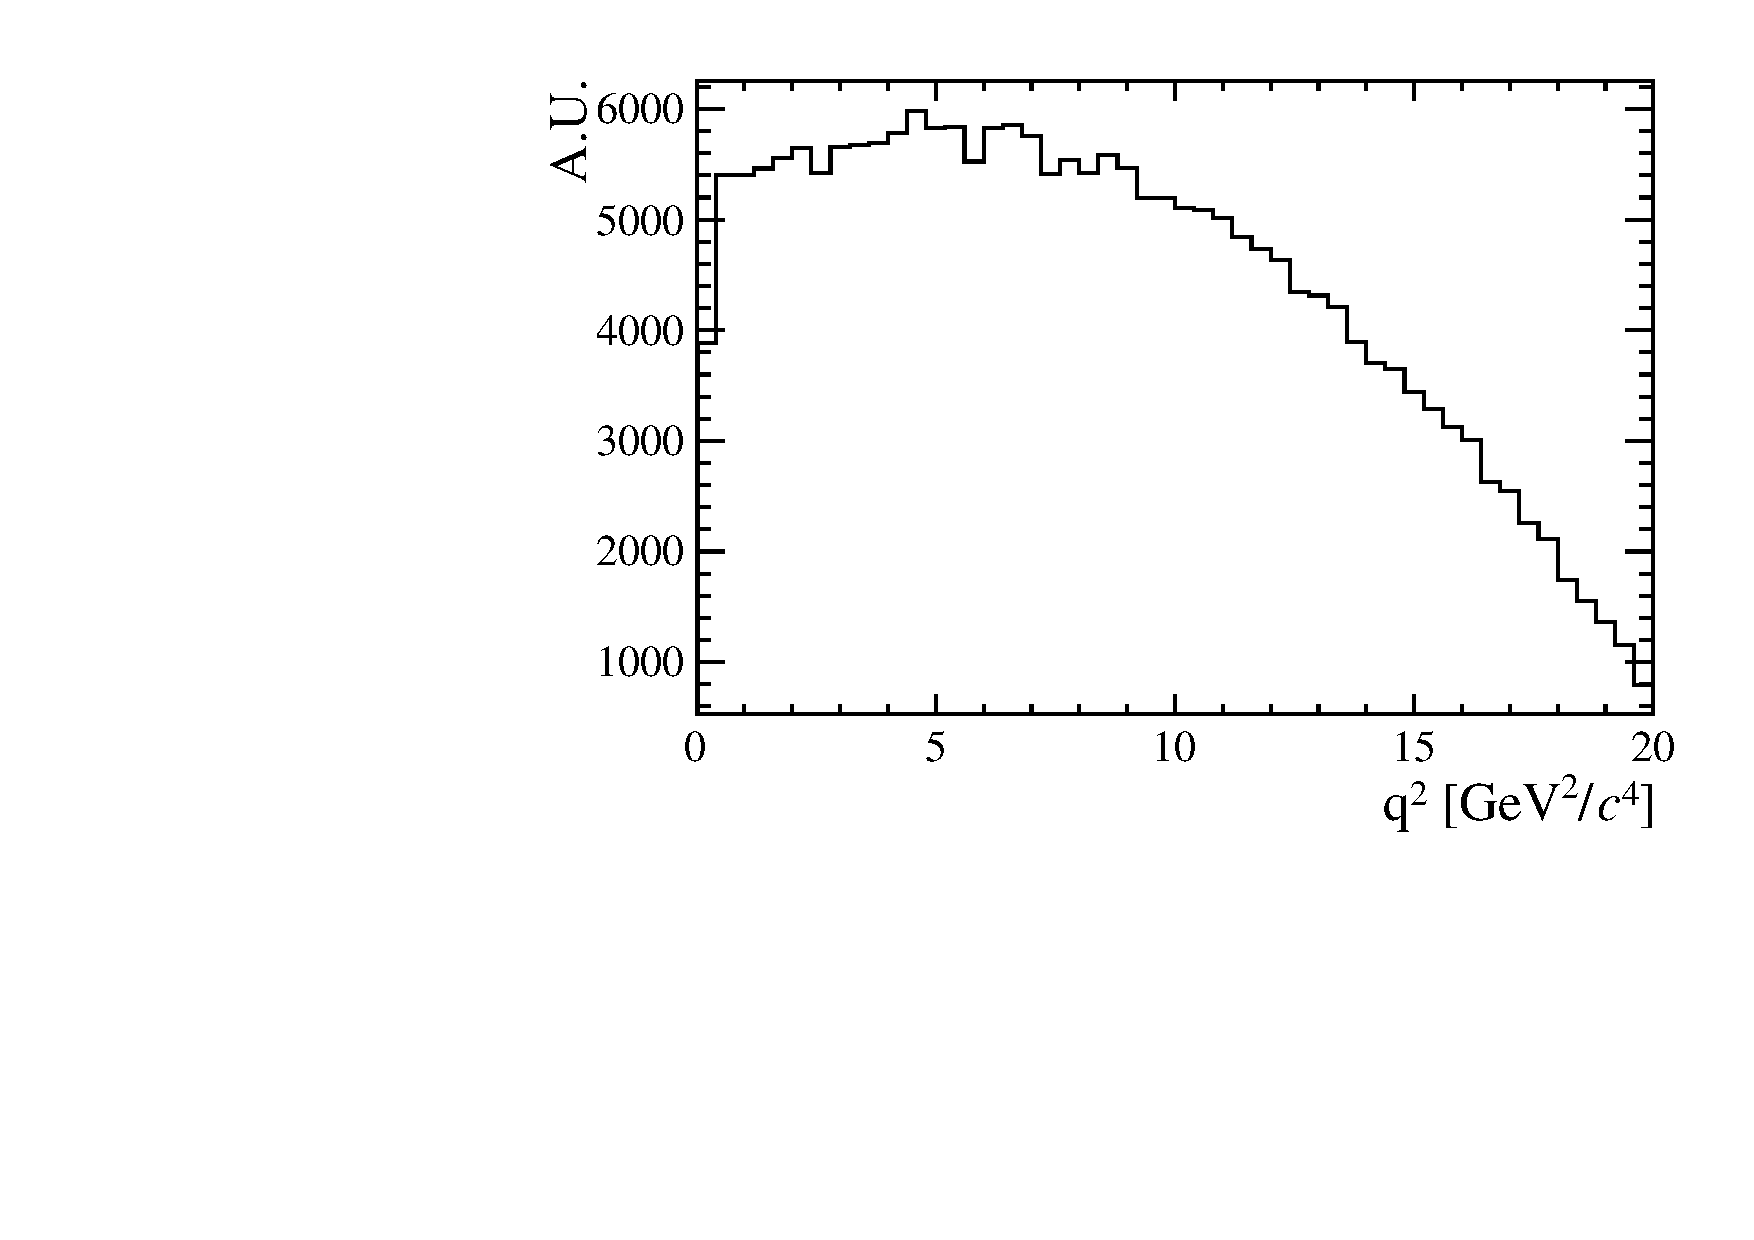
\includegraphics[width=0.48\textwidth]{Lmumu/figs/Q2_beforemodel.pdf}
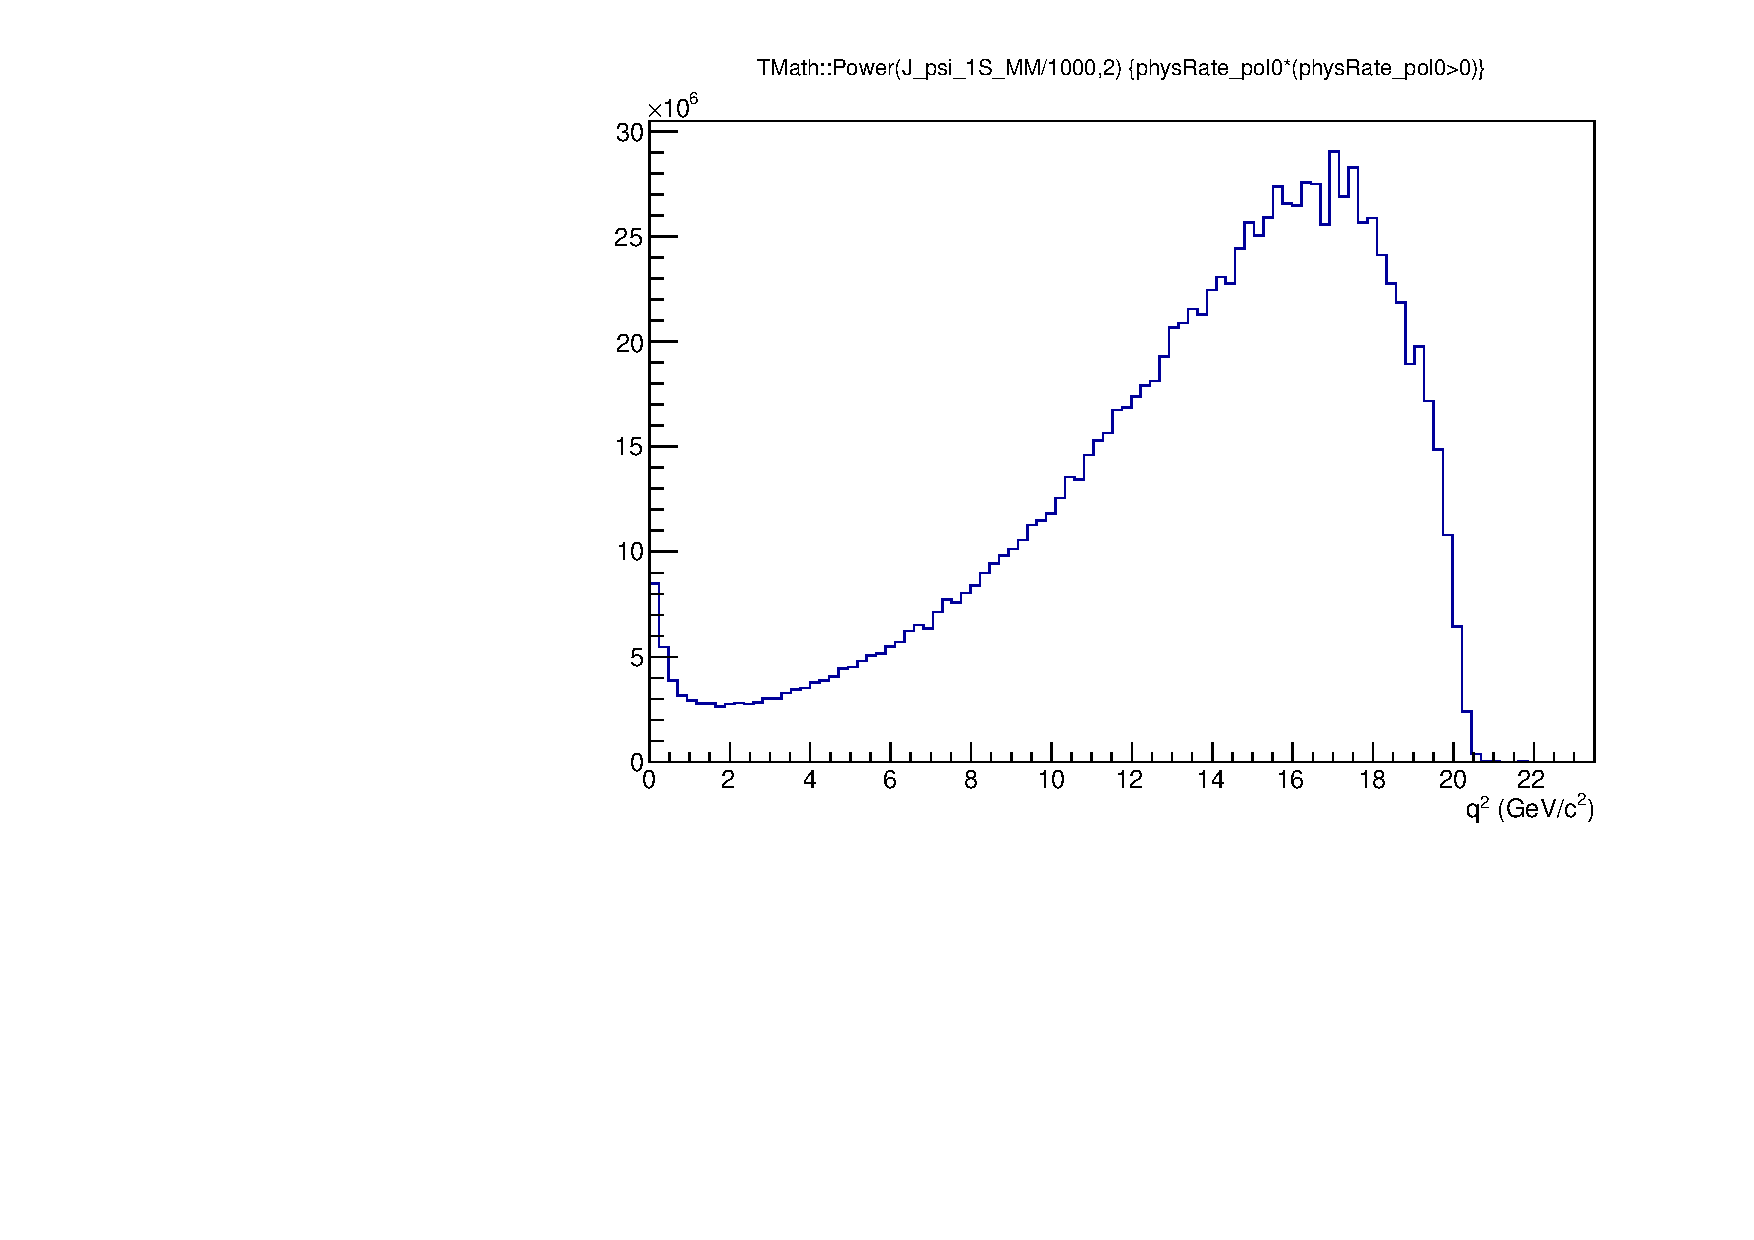
\includegraphics[width=0.48\textwidth]{Lmumu/figs/Q2_aftermodel.pdf}
\caption{The \qsq spectrum of $\Lb\to\Lz\mumu$ simulates events according to the
phase space of the decay (left) and re-weighted using the decay amplitudes (right).}
\label{fig:decaymodeleffonq2}
\end{figure}
%
For the normalisation mode, the decay model used is described in Appendix~\ref{ap:LbJpsiLAngular},
with amplitude magnitudes and production polarisation taken from the measurements in
Ref.~\cite{Aaij:2013oxa}. Phases are not yet measured and are therefore set to zero.

\subsection{Kinematic re-weighting}
\label{sec:kinWeight}

Small data-simulation differences are found in the kinematic properties of the mother particle, \Lb,
which also affect the final state particles. The simulation is re-weighted by 
comparing the momentum and transverse momentum of \Lb baryons in 
real and simulated $\Lb\to\jpsi\Lz$ candidates that satisfy the pre-selection (see Sec.~\ref{sec:Lb_selection}).
To do this a high purity data sample is obtained by selecting a narrow invariant mass interval around the \jpsi 
and \Lb peaks; this contains about $4\cdot10^5$ candidates.
The \Lb invariant mass distribution is then fitted to estimate the number of background decays under the peak.
The background fraction, $f_b = B/(S+B)$, is then used to subtract statistically 
the background from the kinematical distributions as described by the equation:
%
\begin{equation}
S(p,\pt) = T(p,\pt) - f_b\cdot B(p,\pt),
\end{equation}
\noindent
where $S(p,\pt)$ is the distribution of pure signal events, which we want to obtain, $T(p,\pt)$ is the total
distribution of signal plus background, namely the distribution of all events in the signal interval,
$5605 < m(p\pi\mumu) < 5635 \mevcc$, and $B(p,\pt)$ is the pure background
distribution obtained using events from the upper sideband, $m(p\pi\mumu) > 5800 \mevcc$.

After the signal distributions have been obtained from data, they are compared with \mbox{$\Lb\to\jpsi\Lz$} simulated events
and a weight, $w(p_{\Lb},\pt_{\Lb})$ is defined by taking the ratio of the two dimensional $(p,\pt)$ distributions.
The result is shown in Fig.~\ref{fig:kinWeight}, while Appendix~\ref{app:MC_data_comp} reports distributions
of sideband subtracted data in the signal and sideband regions together with weighted and unweighted simulated events.
In these plots the momentum and \pt distributions of \Lb baryons match by construction. The re-weighting also improves the agreement 
between the kinematical distributions of all final particles. Small differences remain due to
the finite binning used for the weights calculation. Quality variables, such as the $\chi^2$ of tracks
and vertices, show little dependence on the kinematics and are relatively unaffected by the weighting procedure.

\begin{figure}
\centering
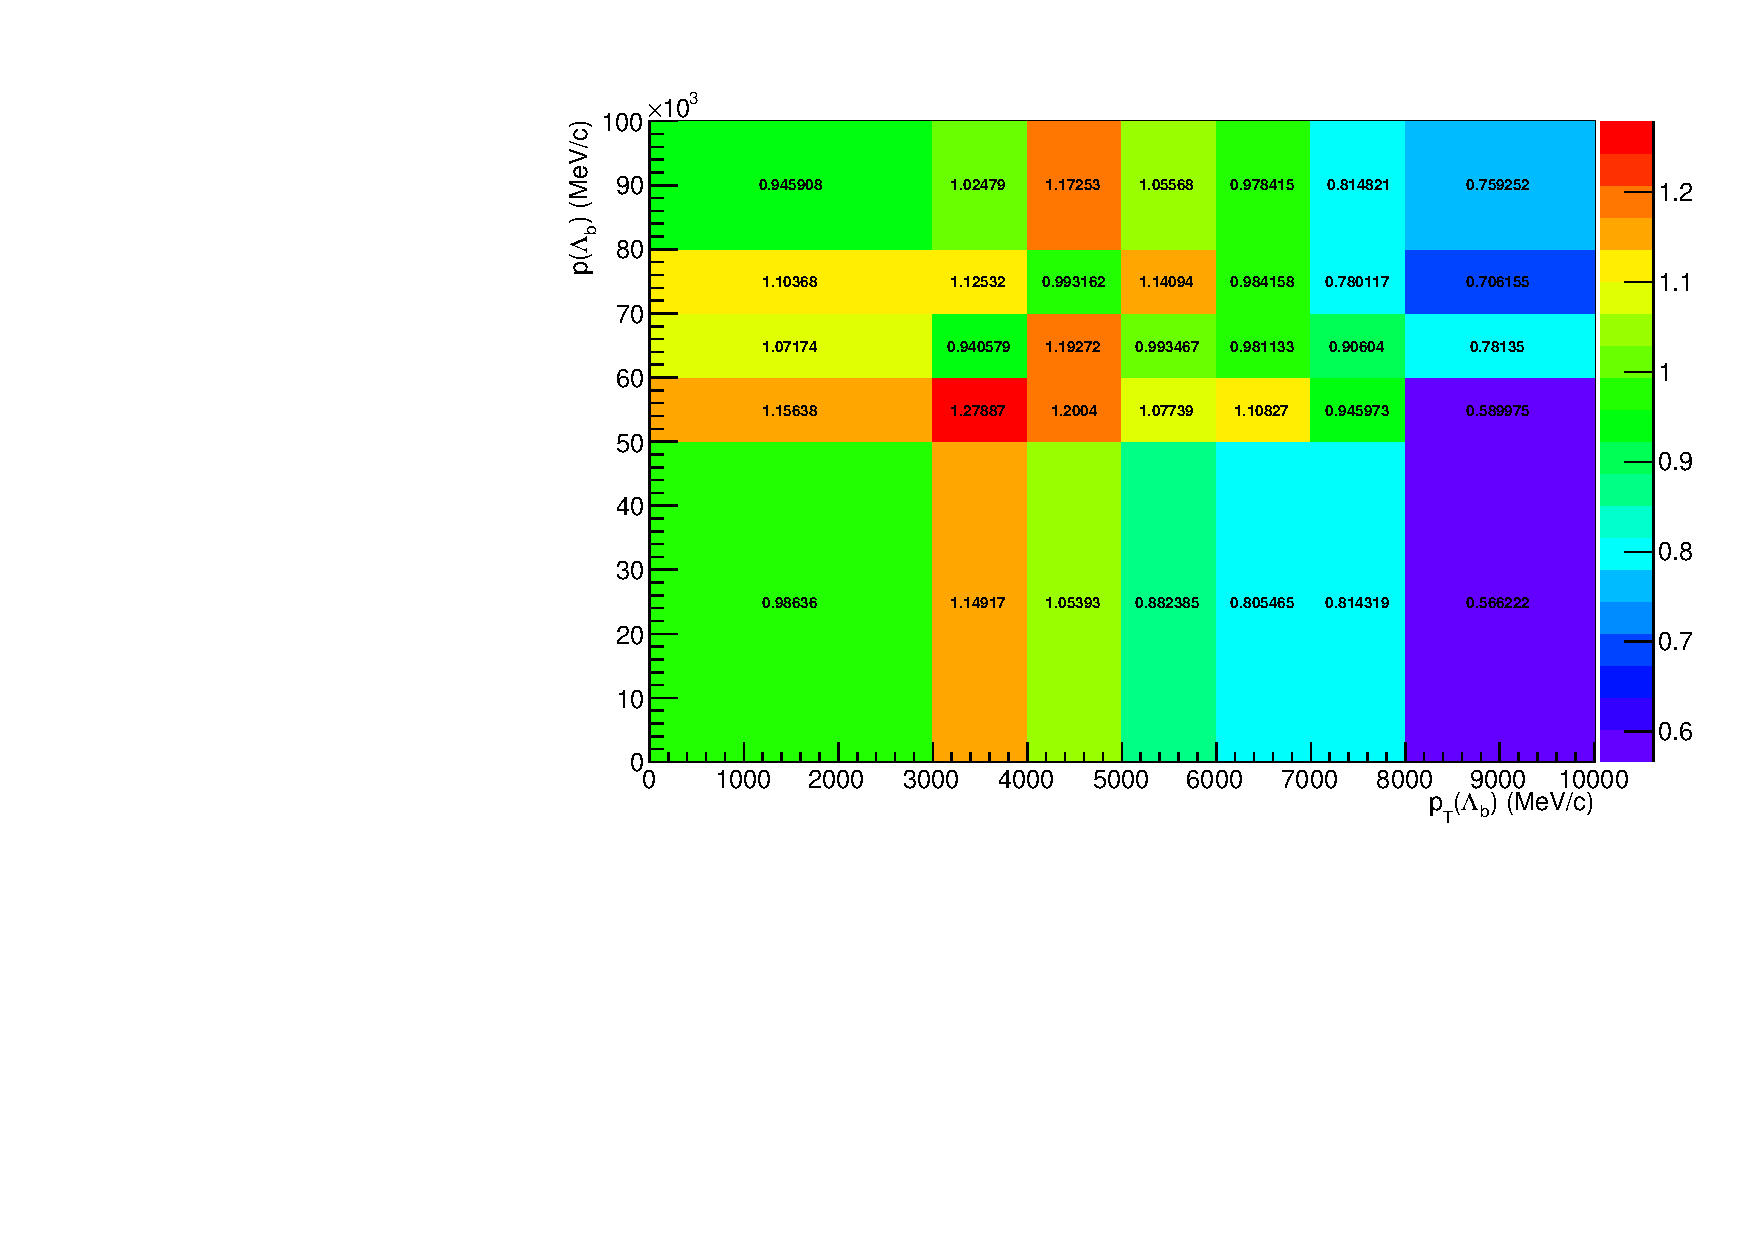
\includegraphics[width=0.9\textwidth]{Lmumu/figs/ratio_Lb_p_pt.pdf}
 \caption{Weights used for the kinematical re-weighting as a function of the momentum and transverse momentum of \Lb. }
\label{fig:kinWeight}
\end{figure}

\subsection{Event type}

There is not complete agreement on the fraction of \Lz baryons reconstructed from long tracks and downstream tracks in data and simulation.
For $\Lb\to\jpsi\Lz$ decays passing the full selection, $\sim 70\%$ of candidates are reconstructed from downstream tracks in data, 
compared with $\sim 75\%$ in the simulation.
The fraction of downstream and long tracks also varies as a function of \qsq and the biggest differences are found at low values of \qsq.
In order to deal with these differences all efficiencies are obtained separately for downstream and long candidates and the analysis is
carried out separately for the two categories; results are then combined to ensure the best use of the available information. 
It is therefore not necessary to correct the simulation to reproduce the correct fraction of events in each category.

